% Source: StudentGovernmentRepo/Common_Sense_Carolina_Lobbying_org/figures/org_phase0.tex
\documentclass[border=5pt]{standalone}
\usepackage{tikz}
\usepackage{xcolor}
\usetikzlibrary{positioning, arrows.meta}

\definecolor{garnet}{HTML}{73000A}
\definecolor{rose}{HTML}{CC2E40}
\definecolor{atlantic}{HTML}{466A9F}
\definecolor{congaree}{HTML}{1F414D}
\definecolor{horseshoe}{HTML}{65780B}

\begin{document}
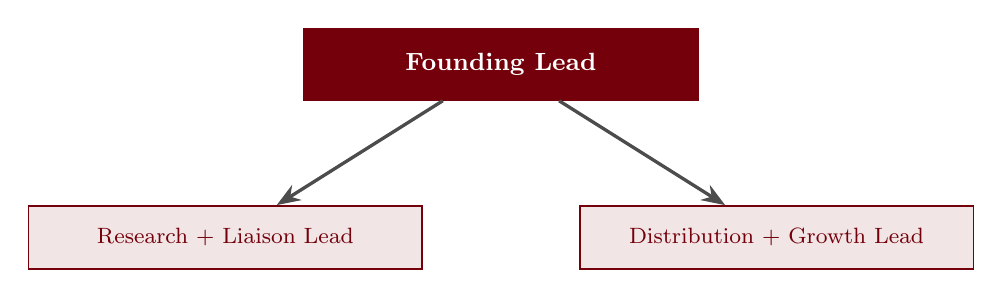
\begin{tikzpicture}[
  every node/.style={rectangle, sharp corners, align=center},
  arrow/.style={-{Stealth[length=3mm]}, line width=1.2pt, black!70}
]

% Top node: Founding Lead
\node[
  fill=garnet,
  text=white,
  draw=garnet,
  line width=0.8pt,
  font=\small\bfseries,
  minimum width=5cm,
  minimum height=0.9cm
] (lead) at (0,0) {Founding Lead};

% Bottom-left node: Research + Liaison Lead
\node[
  fill=garnet!10,
  draw=garnet,
  text=garnet,
  line width=0.6pt,
  font=\footnotesize,
  minimum width=5cm,
  minimum height=0.8cm
] (research) at (-3.5,-2.2) {Research + Liaison Lead};

% Bottom-right node: Distribution + Growth Lead
\node[
  fill=garnet!10,
  draw=garnet,
  text=garnet,
  line width=0.6pt,
  font=\footnotesize,
  minimum width=5cm,
  minimum height=0.8cm
] (distrib) at (3.5,-2.2) {Distribution + Growth Lead};

% Arrows
\draw[arrow] (lead) -- (research);
\draw[arrow] (lead) -- (distrib);

\end{tikzpicture}
\end{document}
